\section{Fundamentação Teórica}

\begin{slide}{Princípios da Destilação por Membranas}
  \footnotesize
  \begin{columns}
    \begin{column}{.58\linewidth}
      \begin{Item}
        \item Processo de separação térmico com membrana \textbf{hidrofóbica} e \textbf{porosa}
        \item Força motriz: \textbf{gradiente térmico} $\rightarrow$ diferença de pressão parcial de vapor
        \item Apenas a fase vapor atravessa os poros da membrana
        \item Mecanismo: evaporação na interface quente $\rightarrow$ difusão nos poros $\rightarrow$ condensação no lado frio
        \item \textbf{Vantagens do processo MD}: opera em temperaturas médias (60--80\,°C), compatível com calor residual e projetos de cogeração; elevada tolerância à salinidade — adequada para soluções de alta concentração onde a osmose inversa é limitada pela pressão osmótica
      \end{Item}
    \end{column}
    \begin{column}{.4\linewidth}
      \centering
      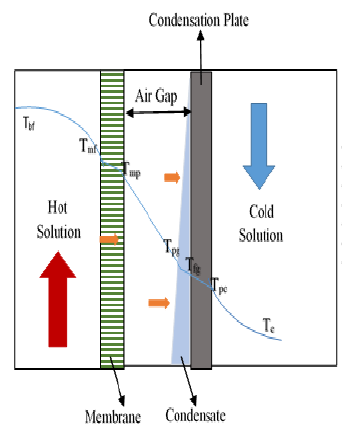
\includegraphics[width=0.72\linewidth]{tcc_images/chap03/Model-of-heat-and-mass-transfer-in-the-AGMD.png}\\[4pt]
      {\tiny Figura: Transporte de calor e massa na configuração AGMD. Fonte: Zheng (2017)}
    \end{column}
  \end{columns}
  \note{A destilação por membranas é um processo térmico onde a água salgada aquecida evapora na interface de uma membrana hidrofóbica e microporosa, o vapor atravessa os poros e condensa do lado frio. Não é filtração — a membrana não é molhada. As vantagens são do processo MD em geral. [~1 min]}
\end{slide}
%========================================================================

\begin{slide}{Fundamentos de Aprendizado de Máquinas}
  \footnotesize
  \vspace{-0.15cm}
  \centering
  \scriptsize
  \begin{tabular}{p{0.17\linewidth} p{0.38\linewidth} p{0.38\linewidth}}
      \toprule
      \textbf{Conceito} & \textbf{Definição} & \textbf{Propósito na Regressão} \\
      \midrule
      \textbf{Métricas}
      & RMSE (raiz do erro quadrático médio), R²
      & RMSE: magnitude do erro na mesma unidade; R²: proporção da variância explicada
      \\
      \midrule
      \textbf{Divisão dos dados}
      & Hold-out (80/20): separar treino, validação e teste
      & Evitar contaminação entre ajuste e avaliação \\
      \midrule
      \textbf{Busca de Hiperparâmetros}
      & Grid Search / Randomized Search sobre espaço de configurações
      & Encontrar a combinação de parâmetros que minimiza o erro de validação \\
      \midrule
      \textbf{Validação Cruzada}
      & Repetir a divisão em partições (K-fold) sem vazamento treino/validação
      & Estimar estabilidade do erro entre partições distintas \\
      \midrule
      \textbf{Validação por Grupos}
      & GroupKFold: mantém dados do mesmo \textbf{grupo} na mesma partição (diferente do K-fold tradicional, que mistura grupos)
      & Avaliar capacidade de extrapolação para grupos não vistos no treino \\
      \midrule
      \textbf{Pré-processamento}
      & Z-score (padronização para média zero e variância unitária)
      & Colocar variáveis em escala comparável, evitando que magnitudes distintas dominem o ajuste \\
      \midrule
      \textbf{Correlação}
      & \textbf{Pearson} ($r$): relação \textit{linear}. \textbf{Spearman} ($\rho$): relação \textit{monotônica}
      & Identificar relações lineares ou monotônicas entre entradas e saídas \\
      \bottomrule
    \end{tabular}
  \note{Campo: regressão supervisionada — prever saídas contínuas (fluxo, temperaturas) a partir de entradas operacionais. 1) Métricas, como medir. 2) Divisão: como separar treino e teste (80/20). 3) Busca de HP: otimização da configuração. 4) Validação cruzada: repetição da divisão para estimar estabilidade. 5) Validação por grupos: grupos inteiros ficam na mesma partição (diferente do K-fold tradicional), avaliando extrapolação. 6) Pré-processamento. 7) Correlação Pearson/Spearman: relações lineares e monotônicas. [~1,5 min]}
\end{slide}

%========================================================================

\begin{slide}{Famílias de Modelos I — Regressão Linear e Regularizadas}
  \centering
  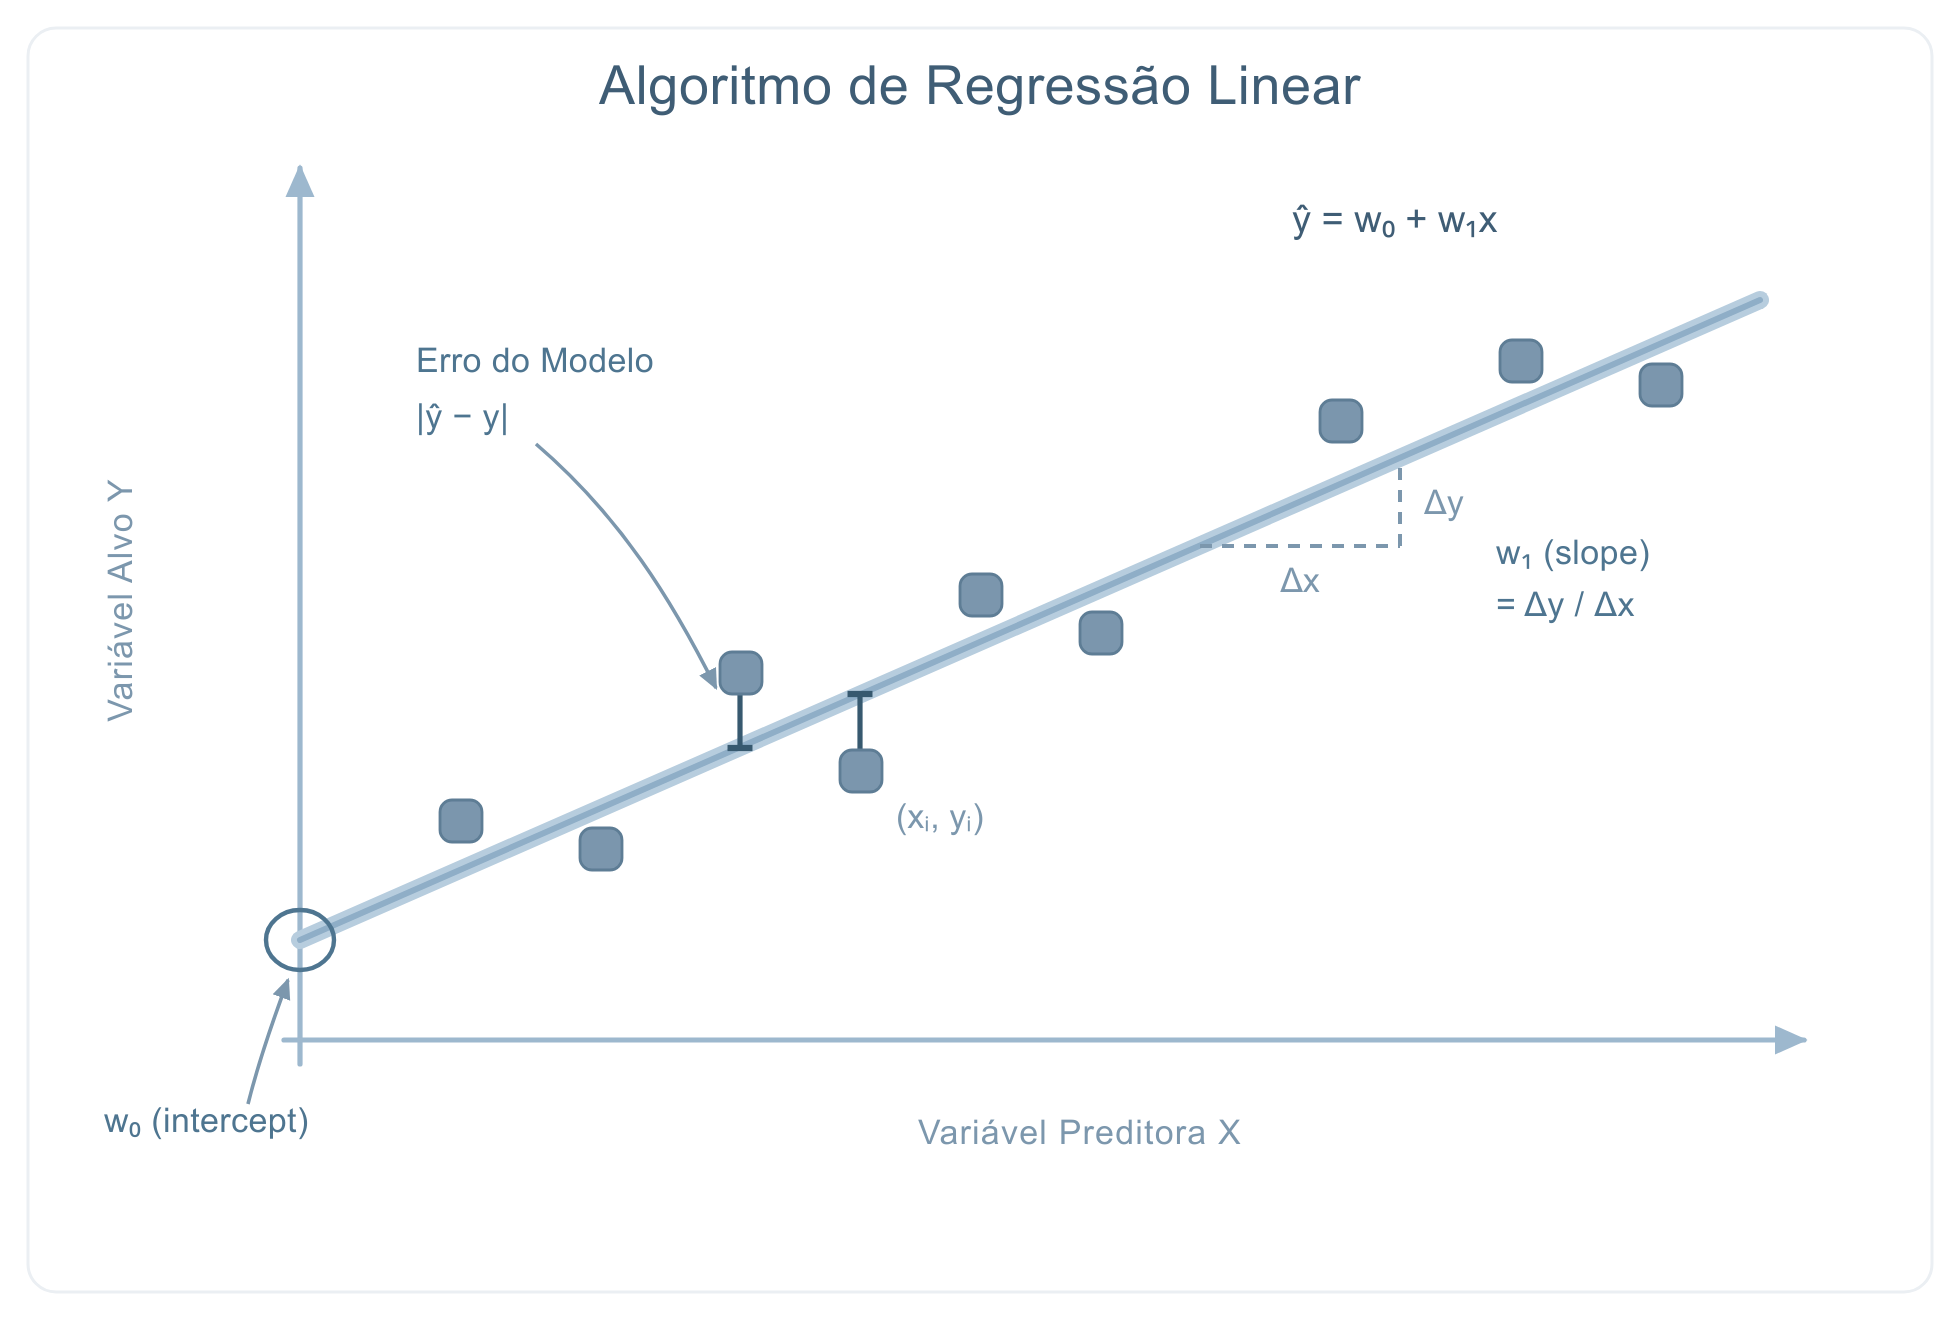
\includegraphics[width=0.62\textwidth]{tcc_images/chap02a/regressao.png}
  \vfill
  {\scriptsize Fonte: Autor}
  \note{Lineares: OLS sem regularização, Ridge penaliza L2 (encolhe coeficientes), Lasso penaliza L1 (zera coeficientes — seleção de variáveis), ElasticNet combina ambos. [~45s]}
\end{slide}
%========================================================================
\begin{slide}{Famílias de Modelos II — Árvores de Decisão}
  \centering
  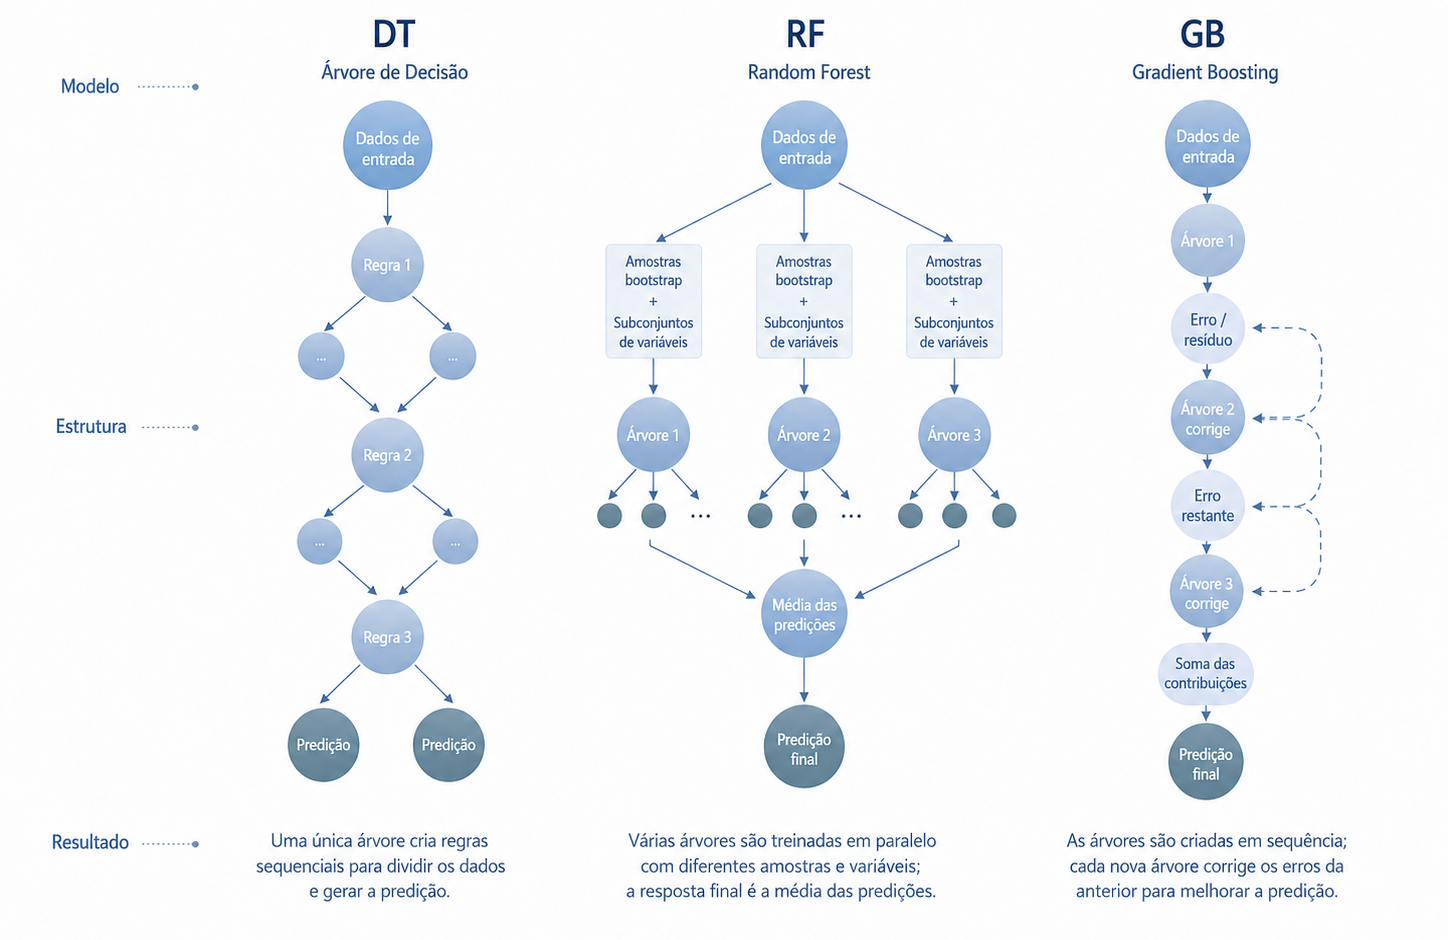
\includegraphics[width=0.68\textwidth]{tcc_images/chap02a/arvores.png}
  \vfill
  {\scriptsize Fonte: Autor}
  \note{Árvores: DT overfitta, RF reduz variância com bagging, GB corrige resíduos sequencialmente. [~45s]}
\end{slide}
%========================================================================
\begin{slide}{Famílias de Modelos III — Redes Neurais}
  \centering
  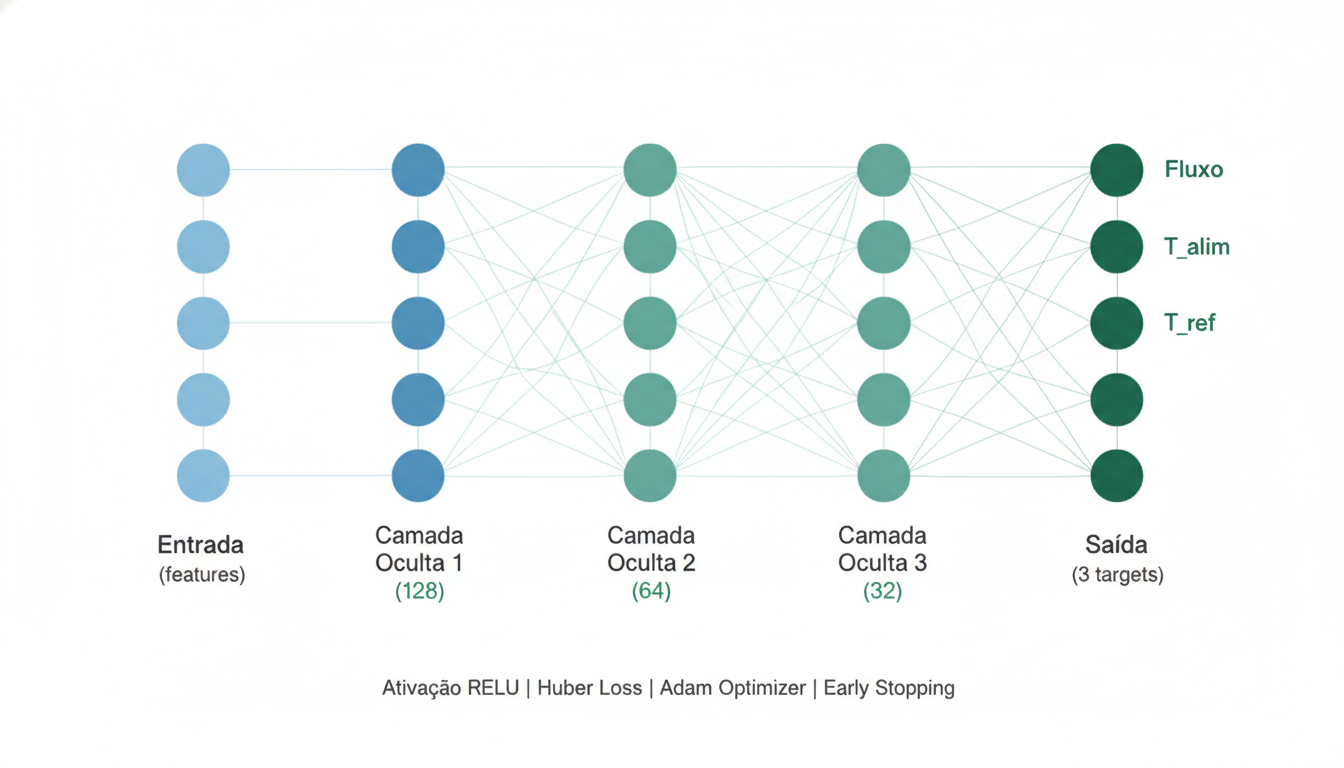
\includegraphics[width=0.78\textwidth]{tcc_images/chap02a/redes_neurais.png}
  \vfill
  {\scriptsize Fonte: Autor}
  \note{MLP: camadas totalmente conectadas, com backpropagation para ajuste dos coeficientes. Hiperparâmetros: camadas, neurônios, ativação, lr, L2. [~45s]}
\end{slide}
%========================================================================
\begin{slide}{Famílias de Modelos IV — Arquiteturas Híbridas}
  \centering
  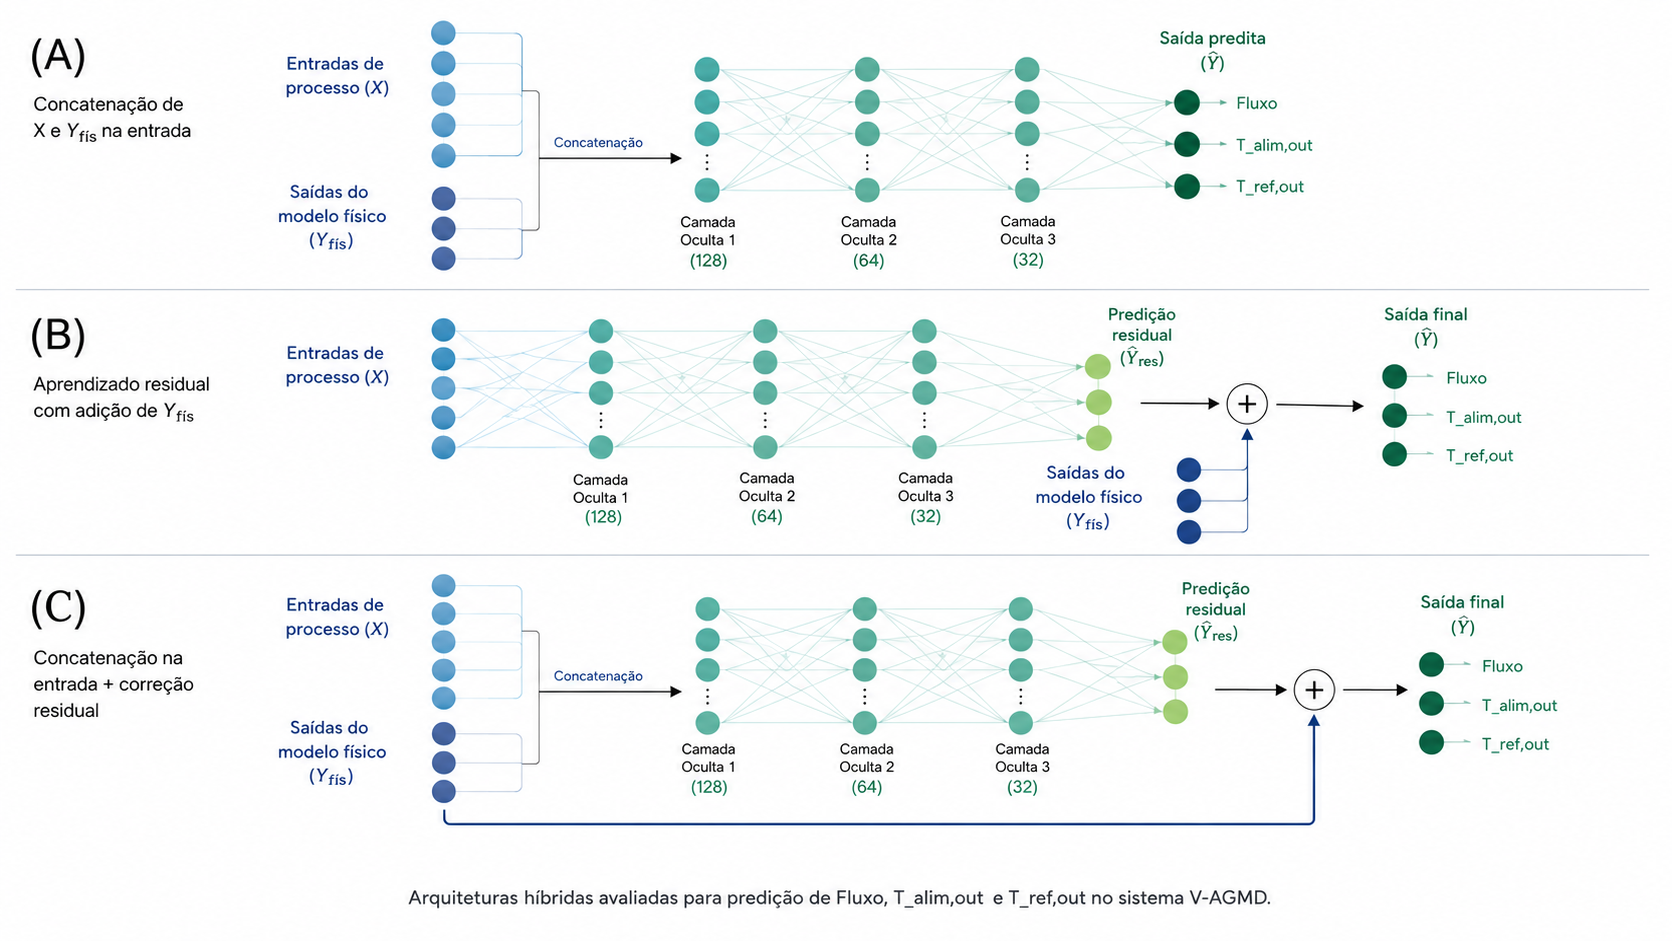
\includegraphics[width=0.78\textwidth]{tcc_images/chap02a/hibridos-slides.png}
  \vfill
  {\scriptsize Fonte: Autor}
  \note{Híbridos: quatro arquiteturas que incorporam o modelo físico 0D. [~30s]}
\end{slide}
%========================================================================


